\section{Additional information about dataset used or estimation methodology}

\subsection{A general description and depiction of convolution}
\label{sec:convol}

In general, the goal of convolution is to propagate the input signal forward in time using a distribution of probabilities. In the 2D and discrete context, it is simply the elementwise multiplication of the signal for some time by a forward-facing distribution of probabilities, which are then summed to get a value for the outcome. Figure~\ref{fig:convol} presents a depiction of the convolution procedure for the signal of smoothed cases (orange line). Essentially, to push the cases forward in time, we take the appropriately aligned (forward-in-time) delay distribution and convolve or multiply the case counts by it to get the distribution of convolved case estimates (blue line). This process is repeated as we march forward in time, as shown through the stop-motion panels, such that it eventually covers the entire line of cases. An important takeaway from this is that convolution is not the same as a simple shift of the data points, but rather it utilizes the most relevant probabilities to propagate the data points forward in time. Deconvolution proceeds in the same fashion, but in the opposite direction to go back in time. 

\begin{figure}[H]
\centering
    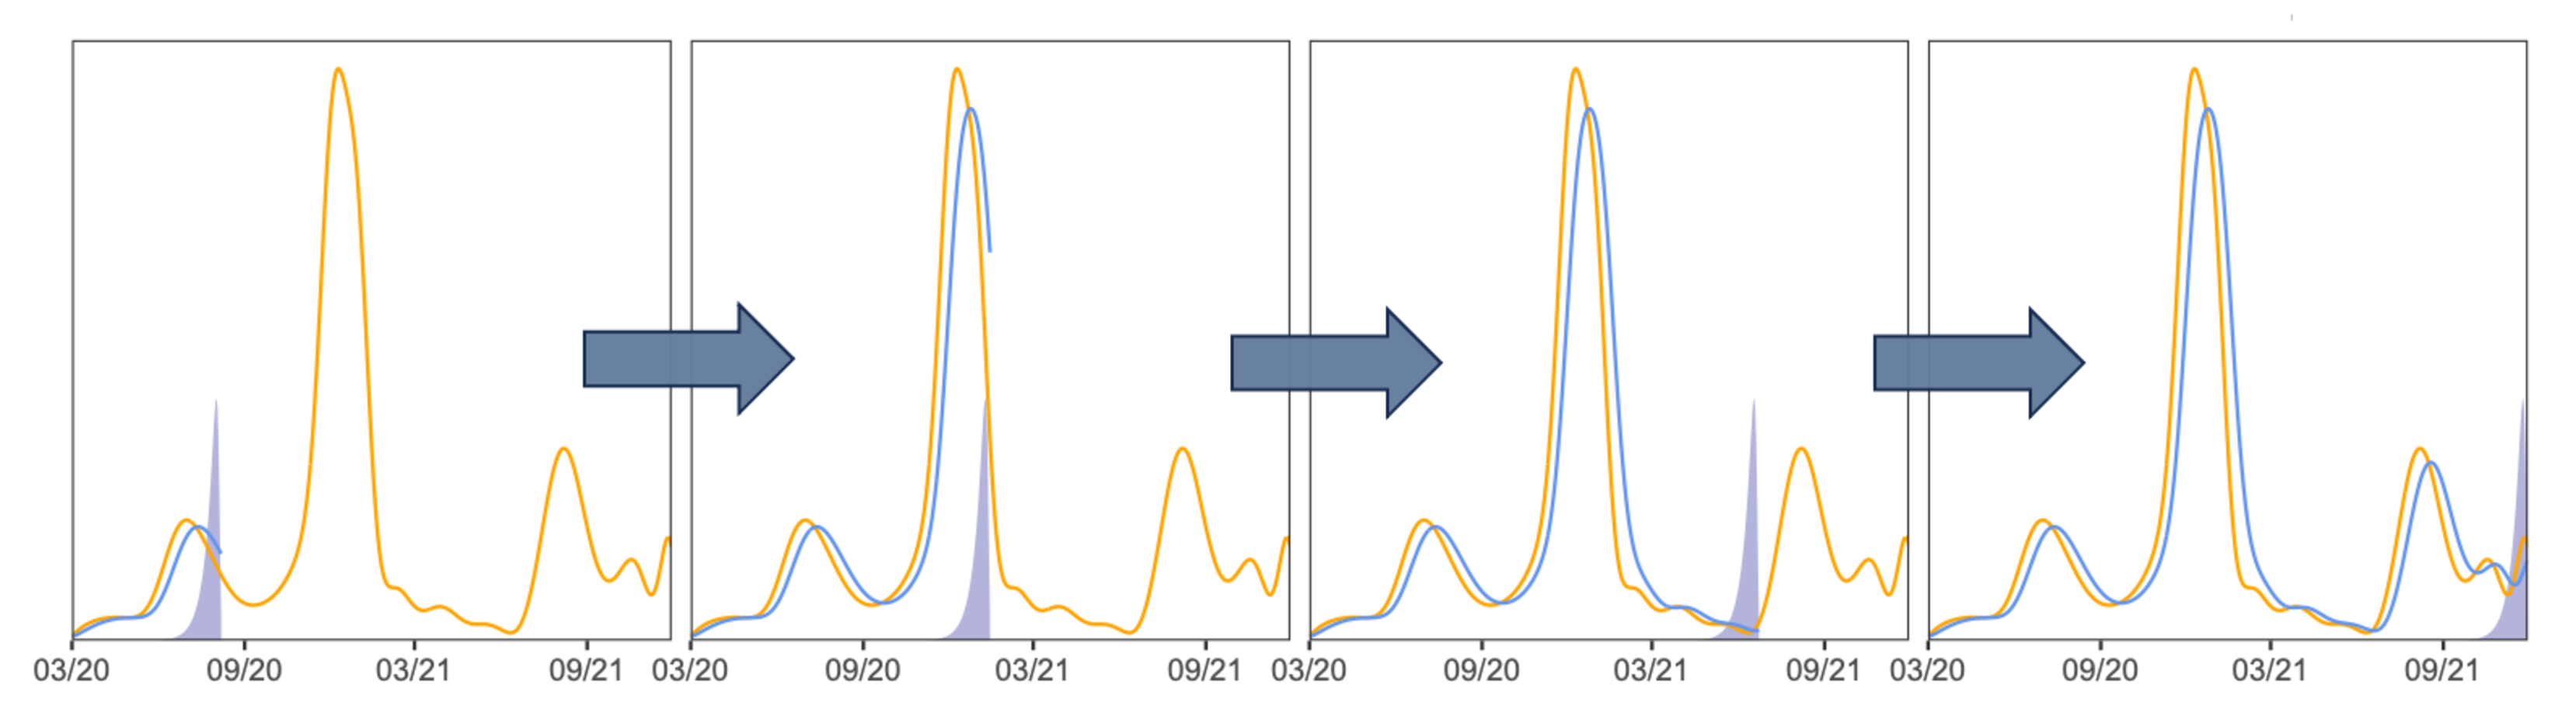
\includegraphics[width=0.99\linewidth]{convolution_diagram.pdf}
    \caption{A general depiction of convolving smoothed cases (orange line) with the corresponding delay probabilities (shaded blue area) to get the convolved estimates (blue line) over four different times.}
    \label{fig:convol}
\end{figure}

\subsection{Additional details on the date fields in the CDC line list}
\label{sec:linelist-details}

Since the restricted dataset is updated
monthly and cases may undergo revision, we use a single version of it that was
released on June 6, 2022. We consider this version to be finalized in that it
well-beyond our study end date such that the dataset is unlikely to be subject
to further significant revisions.

\autoref{tab:order_events_table} presents the percent of pairwise occurrences
for the different possible permutations of events in the line list. Essentially,
most cases follow the idealized ordering shown by
\autoref{fig:chain_events_onset_report} and so we adhere to this construction as
much as possible.

We observe that the line list is prone to high percentages of missing data,
notably with respect to our variables of interest. Approximately 62.3\% of cases
are missing the symptom onset date, 55.4\% are missing positive specimen date,
and 8.96\% of cases are missing the report date. Relatedly,
cases with
missing report or positive specimen dates may be filled with their symptom onset date
\citep{jahja2022real}. So it is possible that all three variables may be
imputed with the same date for a case. However, we only actually deal with
select pairs of events; we do not use all three at once in our construction of
the delay distributions or anywhere else in our analysis. Therefore, we restrict
our investigation of missingness to the pairs of events.
\autoref{fig:prop-cc} suggests that this issue impacts states
differentially due to the inconsistent proportions of zero delay between
positive specimen and report date across states. 

Due to the contamination in the zero delay cases (the true extent of which is
unknown to us), we omit all such cases where the positive specimen and report
dates have zero delay from our analysis. We choose to allow for zero and
negative delay for symptom onset to report because correspondence with the CDC
confirms the distinct possibility that a person could test positive before
symptom onset and it is a reasonable ordering to expect if, for example, the
individual is aware that they have been exposed to an infected individual.

\begin{figure}[!tb]
\centering
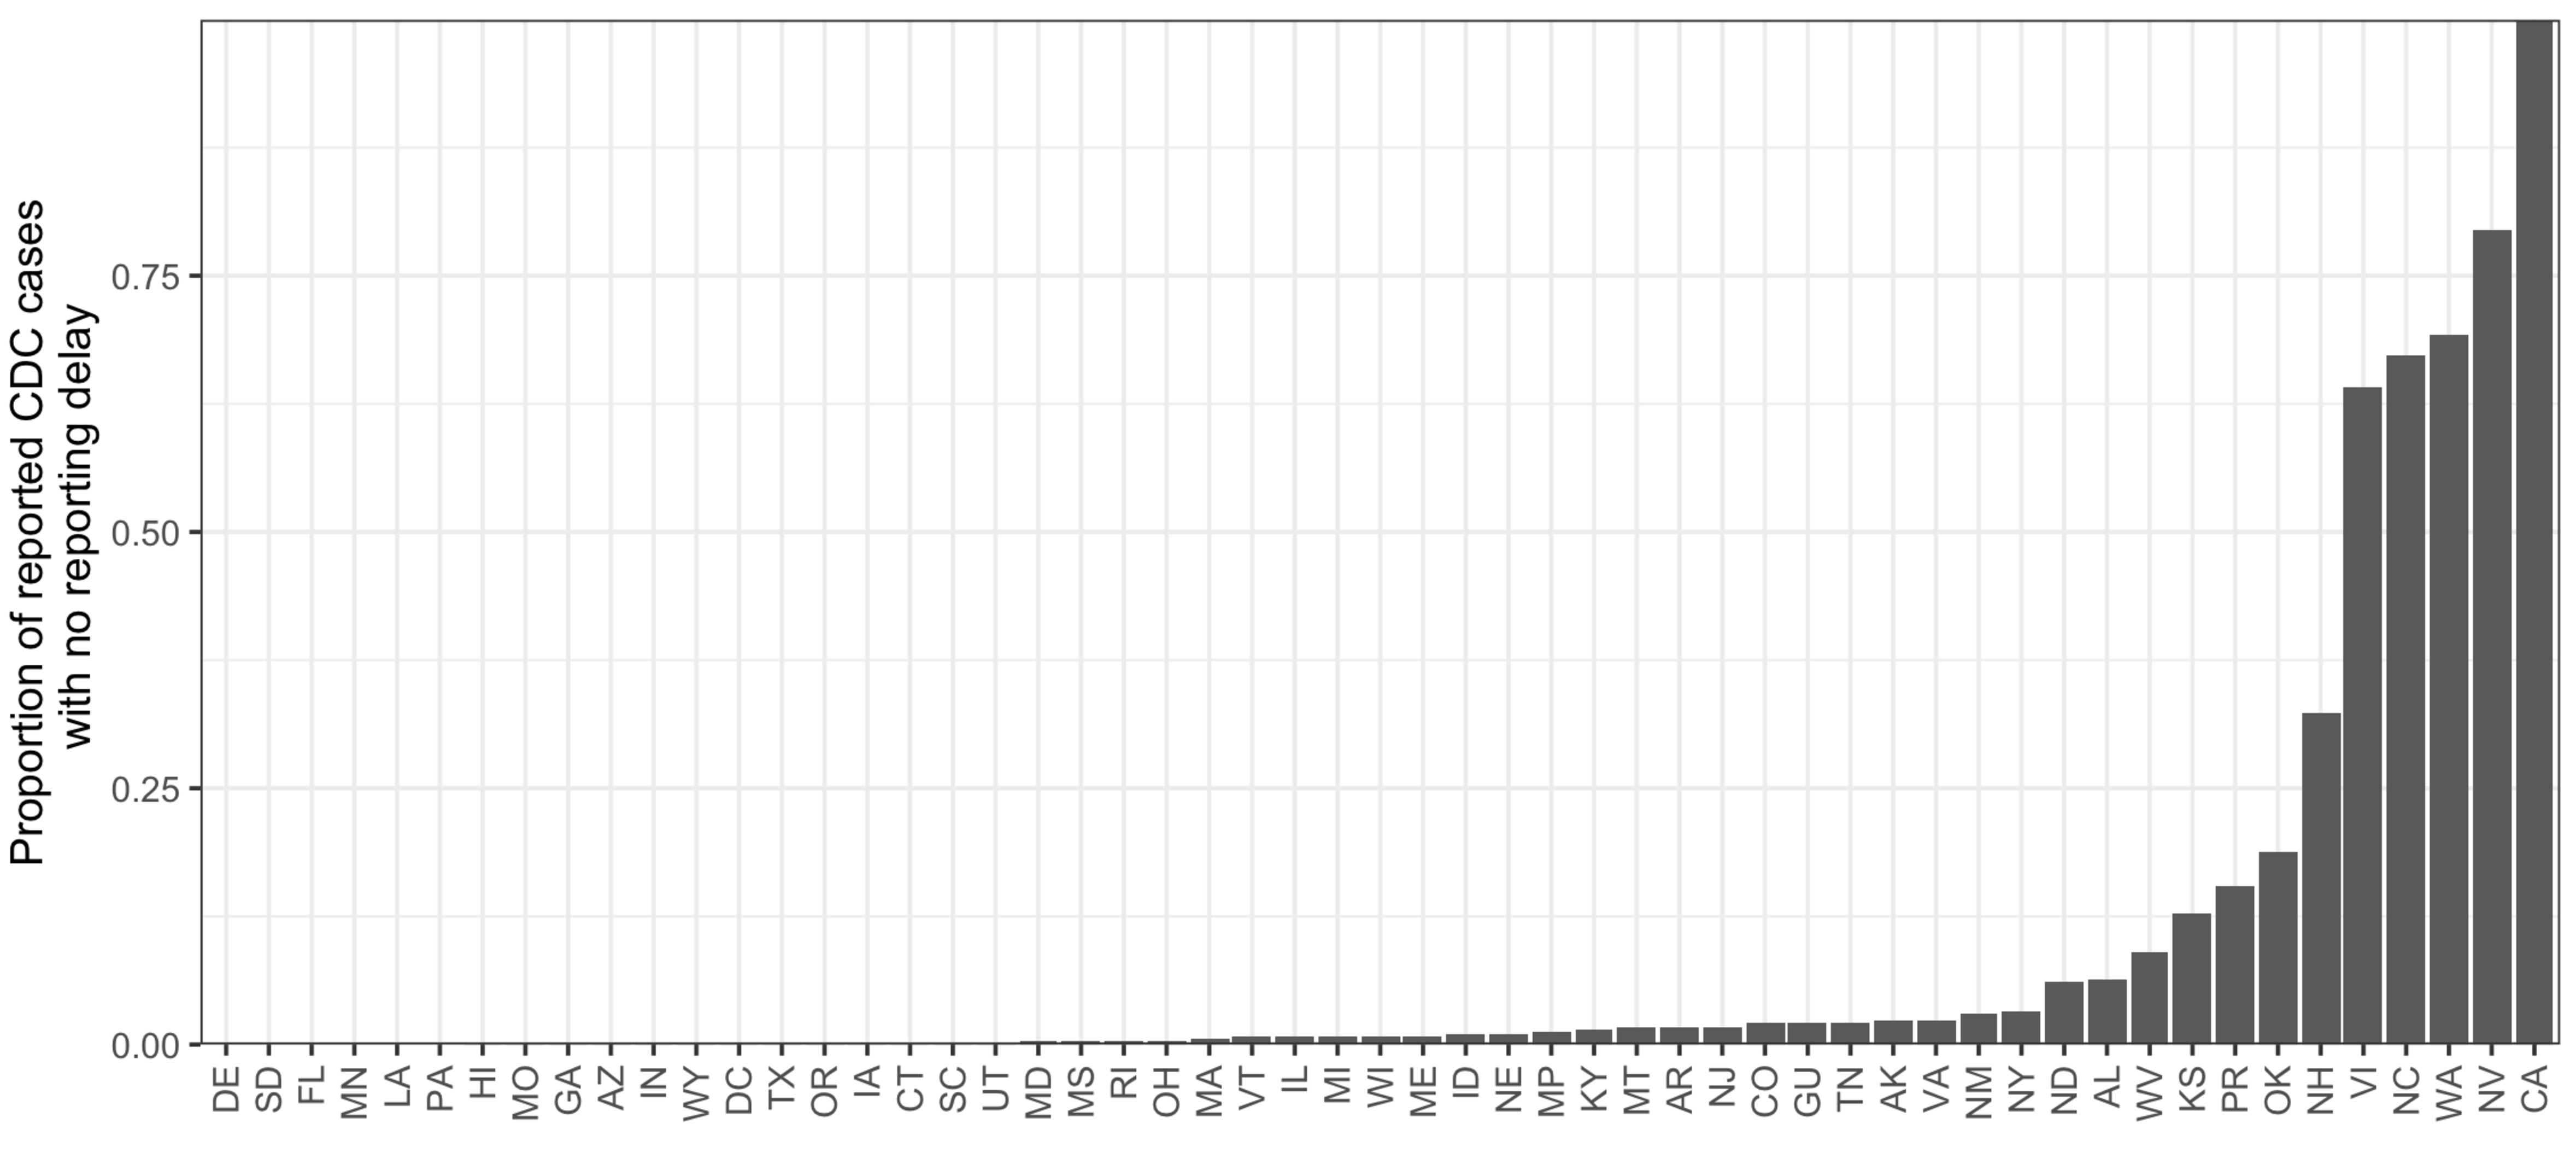
\includegraphics[width=0.9\linewidth]{prop_cc_zero_delay.pdf}\\
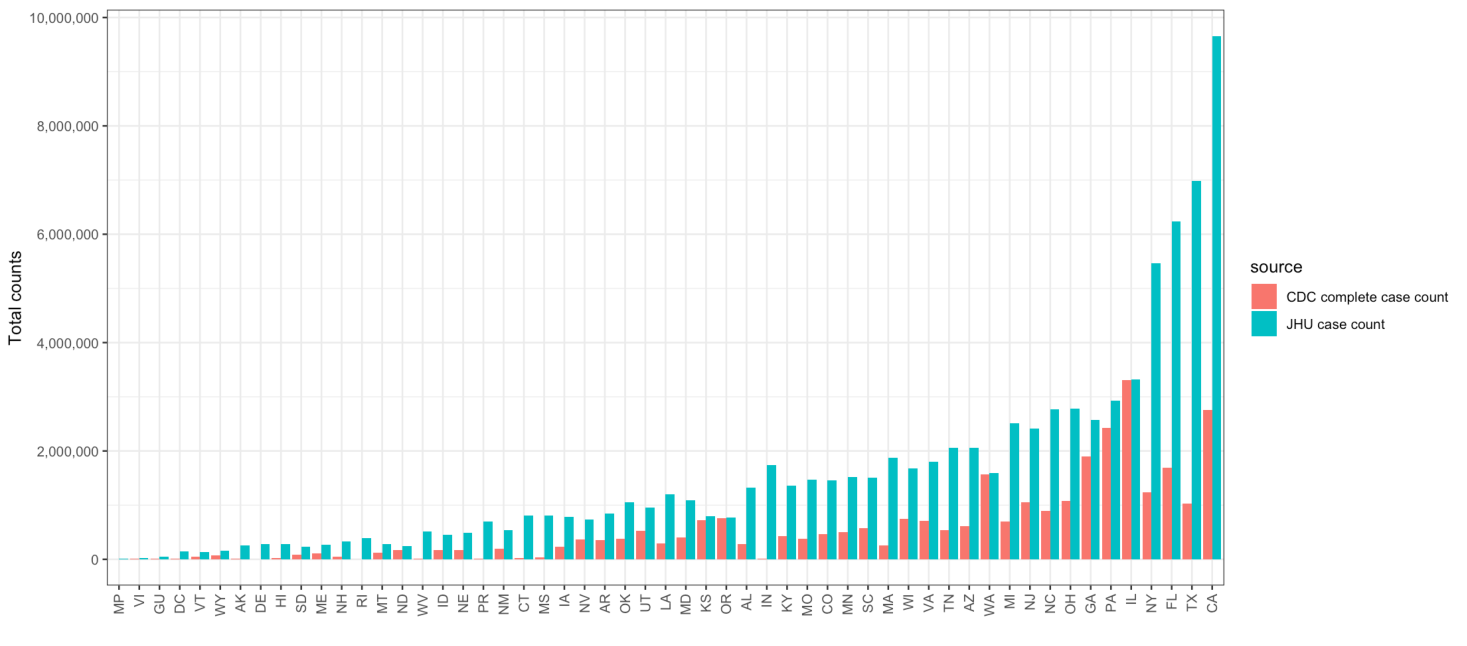
\includegraphics[width=0.9\linewidth]{prop_cc_cdc_vs_jhu.pdf} 
\caption{Top panel: Proportion of complete cases with zero delay between
    positive specimen and report date in the restricted CDC line list dataset.
    Bottom panel: Complete case counts by state in the CDC line list versus the
    cumulative complete case counts from JHU CSSE as of June 6, 2022. All
    counts have been scaled by the 2022 state populations as of July 1, 2022
    from \citep{uscensus2022annual}.}
\label{fig:prop-cc}
\end{figure}

For the same release date, the restricted line list contains 74,849,225 cases
(rows) in total compared to 84,714,805 cases reported by the JHU CSSE; that is,
line list is missing about 10 million cases. The extent that this issue impacts
each state is shown in \autoref{fig:prop-cc}, from which it is clear
the fraction of missing cases is substantial for many states, often surpassing
50\% \citep{jahja2022real}. In addition, the probability of being missing does
not appear to be the same for states, so there is likely bias introduced from
using the complete case line list data. We consider such bias to be unavoidable
in our analysis due to a lack of alternative line list sources.

In the line list, we observe unusual jarring spikes in reporting in 2020
compared to 2021. Upon plotting by report date, we find that a few states are
contributing unusually large case counts on isolated days very late in the
reporting process (usually well beyond 50 days). We strongly suspect that these
large accumulations of cases over time are due breakdowns of the reporting
pipeline (which may be expected to occur more frequently in the year following
its instantiation than later in time). Such anomalies are not likely to be
reliable indicators of the delay from positive specimen to case report.
Therefore, we devise a simple, ad hoc approach to detect and prune these
reporting backlogs.

First, we obtain the part of the line list intended for the positive specimen to
case report delay estimation, where both such dates are present and where zero
and negative delay cases have been omitted. Then, for each of the three dates of
June 1, September 1, and December 1, 2020, we bin the reporting delays occurring
from 50 days up to the maximum observed delay. For each bin, we obtain the total
delay count for each state. We check whether each count on the log scale is at
least the median (for the bin) plus 1.5 times the interquartile range and retain
only those that exceed this criterion as potential candidates for pruning. Next,
we compute the counts by report date for each candidate state. If there is a
report date with a count greater than or equal to the pre-specified threshold,
then we remove those cases from the line list. Based on inspection and
intuition, we set the threshold to 2000 for the first two bins, and then lower
it to 500 for the remaining bins. A similar trial and error approach is used to
set the bin size (to 50 days).

\subsection{Table on the percent pairwise occurrence of events in the CDC line list}
\begin{table}[h!]
\begin{tabular}{|l|l|l|}
\hline
\textbf{Order of events}                              & \textbf{Percent pairwise occurrence}                                                                                    & \textbf{Handling}                                                                                                                                                                                                                                                                                                                                                          \\ \hline
IO $\rightarrow$ SO $\rightarrow$ PS $\rightarrow$ RE & \begin{tabular}[c]{@{}l@{}}PS $\geq$ SO: 97.1 \\ PS = SO: 33.6\\ PS \textgreater RE: 1.74\\  PS = RE: 14.6\end{tabular} & \begin{tabular}[c]{@{}l@{}}This is the idealized order of events and so we \\ built the current support sets for \\ SO $\rightarrow$ PS and PS $\rightarrow$ RE \\ delay distribution constructions around this \\ such that IO comes first by construction, \\ SO typically precedes PS, but may be the same \\ or come before, and RE comes after PS and SO\end{tabular} \\ \hline
IO $\rightarrow$ PS $\rightarrow$ SO $\rightarrow$ RE & \begin{tabular}[c]{@{}l@{}}PS \textless SO: 2.91 \\ SO $\leq$ RE: 99.3 \\ SO \textless RE: 86.1\end{tabular}            & \begin{tabular}[c]{@{}l@{}}Allowed for negative delays up to the largest \\ non-outlier value for the 0.05 quantile of delay\\ from PS to SO by state\end{tabular}                                                                                                                                                                                                         \\ \hline
IO $\rightarrow$ PS $\rightarrow$ RE $\rightarrow$ SO & \begin{tabular}[c]{@{}l@{}}RE \textless SO: 0.7 \\ RE \textless PS: 1.7\end{tabular}                                    & \begin{tabular}[c]{@{}l@{}}Nothing because current handling of the CDC \\ of the line list ensures that the most concerning \\ cases are handled where \\ SO = PO = RE, SO = RE and PO = RE\end{tabular}                                                                                                                                                                   \\ \hline
\end{tabular}
\caption{Percent pairwise occurrence for the different permutations of events considered in the restricted CDC line list. The abbreviation IO stands for infection onset, SO is symptom onset, PS is positive specimen, and RE is report date. We consider a restricted set of permutations because we assume that IO must come first and that PS must precede report date for a case to be legitimate. Finally, the underlying assumption for the percent pairwise occurrence calculations is that the cases must have both elements present (not missing).}
\label{tab:order_events_table}
\end{table}

\subsection{Justifications for delay distribution calculations}
\label{sec:delay-justifications}

Let $y_t$ denote the count of new cases reported at time $t$ and $x_t$ denote
the count of deconvolved cases with positive specimen at $t$. For all cases in
the line list that had both a positive specimen and a report date, we can count
the those that are reported at time $t$ by enumerating them according to
positive specimen date (similar to how symptom onset date was used in
\citealp{jahja2022real}):
\begin{align*}
y_t = \sum_{s=1}^{t} \sum_{i=1}^{x_s}\indicator \left ( \text{the }i\th\text{ positive specimen at }
    s \text{ gets reported at }t \right ).
\end{align*}
Taking the conditional expectation of the above yields
\begin{align*}
\E(y_t \mid x_s, s \leq t) = \sum_{s=1}^{t} \pi_t(s) x_s ,
\end{align*}
where $\pi_t(s) = \P(\text{case report at }t \mid \text{positive specimen date
at }s)$ for each $s \leq t$ are the delay probabilities and the $\{ \pi_t(s) : s
\leq t \}$ sequence comprises the delay distribution at time $t$. Notice that
there are no time restrictions placed on the positive specimen date, except that
it must have been between the start of the pandemic and the report date,
inclusive. This is unlikely to be a realistic assumption to make as $t$ moves
farther away from $s$. 

Thus, we make three key assumptions about these distributions. First, positive
specimen tests that are reported to the CDC are always reported within $d = 60$
days, which is true for the majority of the reported cases. Second, the
probability of zero delay is zero, which stems from the contamination of
zero-delay in the line list. We update the
conditional expectation formula to reflect these two assumptions as in \citep{jahja2022real}: 
\begin{align*}
\E(y_t \mid x_s, s \leq t) = \sum_{k=1}^{60} p_t(k) x_{t-k}
\end{align*}
where for $k = 1, \dots, 60$,
\begin{align*}
p_t(k) = \P(\text{case report at }t \mid \text{positive specimen at }t-k).
\end{align*}


Thirdly, there are times where the empirical probability
was observed to be precisely 1 at zero delay and the proportion of CDC relative
to JHU cases used for the weight was also 1. Since we believe that having zero
delay for all cases is unrealistic and unlikely to be representative of all
cases for the state, we inject a small amount of variance manually by setting
the the CDC-to-JHU proportion to be the minimum shrinkage proportion observed
for the affected state (such instances were isolated to the state of New
Hampshire). Aside from these modifications, the construction of the delay
distribution proceeds in precisely the same manner as for positive specimen to
report date. 

\subsection{Details about seroprevalence data}
\label{sec:sero-details}

In the former, the CDC
collaborated with 17 blood collection organizations in the largest nationwide
COVID-19 seroprevalence survey to date \citep{cdc2021blood}. The blood donation
samples were used to construct monthly seroprevalence estimates for nearly all
states from July 2020 to December 2021 \citep{jones2021estimated}. In the latter
survey, the CDC collaborated with two private commercial laboratories and used
blood samples to test for the antibodies to the virus from people that were in
for routine or clinical management (presumably unrelated to COVID-19
\citealp{bajema2021estimated}). The resulting dataset contains seroprevalence
estimates for a number of multi-week collection periods starting in July 2020 to
February 2022. 

Both datasets are based on repeated, cross-sectional studies that aimed, at
least in part, to estimate the percentage of people who were previously infected
with COVID-19 using the percentage of people from a convenience sample who had
antibodies against the virus \citep{bajema2021estimated, cdc2020data,
jones2021estimated}. Adjustments were made in both for age and sex to account
for the demographic differences between the sampled and the target populations.
However, both datasets are incomplete and they differ in the number and the
timing of the data points for each state (\autoref{fig:sero_blood_comm_compar}).
Such limitations indicate that reliance upon only one seroprevalence survey is
inadvisable. For example, in the commercial dataset, the last estimate for North
Dakota is in September 2020. In the blood donor dataset, Arkansas does not have
estimates available until October 2020. 

\begin{figure}[!tb]
\centering
    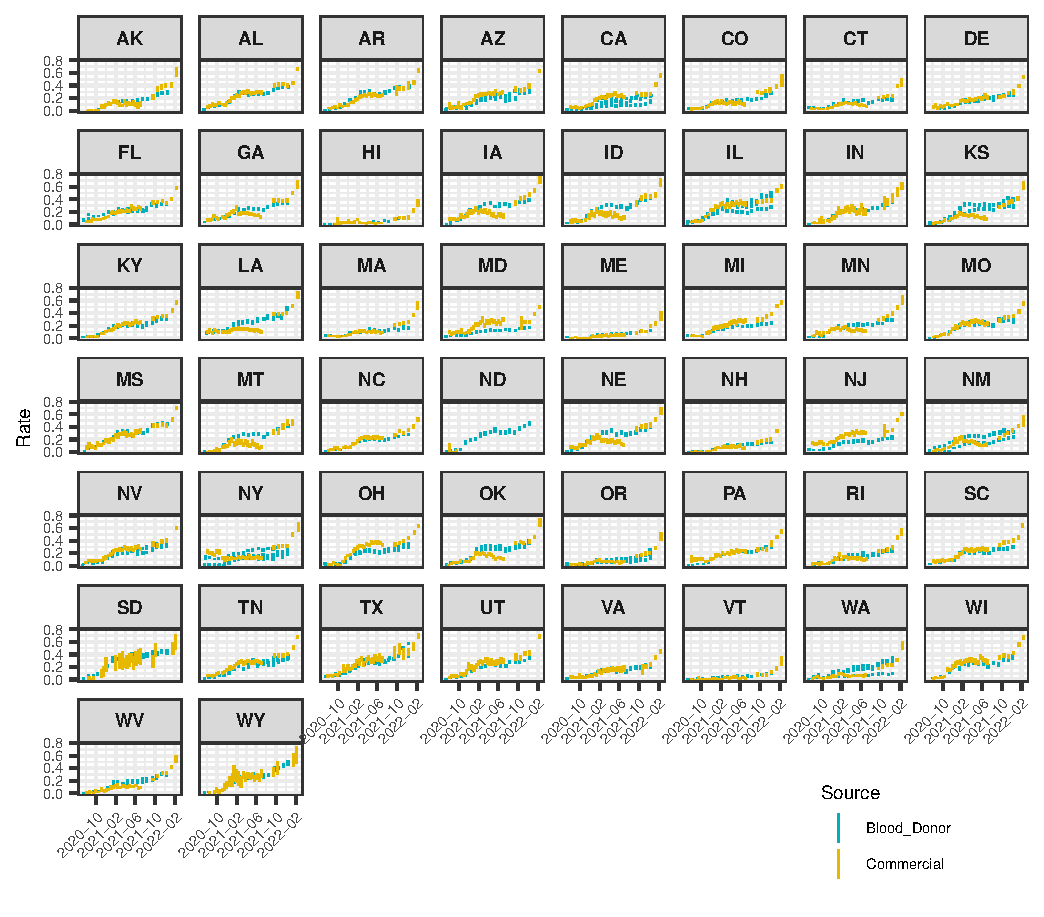
\includegraphics[width=.99\textwidth]{sero_blood_comm_compar.pdf}
    \caption{A comparison of the seroprevalence estimates from the Commercial
    Lab Seroprevalence Survey dataset (yellow) and the 2020--2021 Blood Donor 
    Seroprevalence Survey dataset (blue). Note that the maximum and the minimum
    of the line ranges are the provided 95\% confidence interval bounds to 
    give a rough indication of uncertainty.}
    \label{fig:sero_blood_comm_compar}
\end{figure}
    
The date variables that come with the two seroprevalence datasets are different
and so the date variables that we are able to construct from them are not the
same. For the commercial dataset, we use the midpoint of the provided specimen
collection date variable. A major difference in the structure of the two
datasets is that the commercial dataset always has the seroprevalence estimates
at the level of the state, while the blood donor dataset can either have
estimates for the state or for multiple separate regions within the state. For
the blood donor dataset, we use the median donation date if the seroprevalence
estimates are designated to be for entire state. If they are instead for regions
in the state, since there is reliably one measurement per region per month, we
aggregate the measurements into one per month per state by using a weighted
average (to account for the given sample sizes of the regions). The median of
the median dates is taken to be the date for the weighted average.

To adapt to the sparseness in the seroprevalence data, we convert our daily data
to weekly by summing the reported infections and shifting the observed
seroprevalence measurements to the nearest Monday. If there are multiple
measurements in a week from a seroprevalence source, then the average is used.
We denote these changes by changing the time-based subscript from $t$ to $m$
where $m$ indicates the Monday relative to our June 1, 2020 start date.
Since we operate with weekly data where the weeks are designated by Monday, we set the 
end date to be November 29, 2021. 

\subsection{State space representation of the antibody prevalence model}\label{supp:ssapm} 

The antibody prevalence model from \autoref{eq:waningpr} is conceptualized
as a Gaussian state space model (as in \citealp{durbin2012time, helske2017kfas}).

In general, for $t = 1, \dots, n$, let $\alpha_t$ be the $m \times 1$ vector of
latent state processes at time $t$ and $y_t$ be the $p \times 1$ vector of
observations at time $t$. Under the assumption that $\eta$ is a $k \times 1$
vector, the form of the linear Gaussian state space model is 
\begin{align}
y_t &= Z\alpha_t + \epsilon_t, \qquad \epsilon_t \sim N(0, H_t) \label{eq:ss1}\\
\alpha_{t+1} &= T_t\alpha_t + R_t\eta_t, \quad \eta_t \sim N(0, Q_t) \label{eq:ss2}
\end{align}
where $\alpha_1 \sim N(a_1, P_1)$ and 
there is independence amongst $\alpha_1$, $\epsilon_t$ and $\eta_t$
\citep{helske2017kfas, durbin2012time}. For notational
compactness, we let $\alpha = \left ( \alpha_1^\top, \dots, \alpha_n^\top \right )$
and $y = \left ( y_1^\top, \dots, y_n^\top \right )$.

The observation equation can be viewed as a linear regression model with the
time-varying coefficient $\alpha_t$, while the second equation is a first-order
autoregressive model, which is Markovian in nature \citep{durbin2012time}. 

The underlying idea behind the two equations is that we are assuming that the
system evolves according to $\alpha_t$ (as in the second equation), but since
those states are not directly observed, we turn to the observations $y_t$ and
use their relationship with $\alpha_t$ (as in the first equation) to drive the
system forward \citep{durbin2012time}. So the objective of state space modeling
is to obtain the latent states $\alpha$ based on the observations $y$ and this
is achieved through Kalman filtering and smoothing. 

Kalman filtering gives the following one-step-ahead predictions of the states
\begin{align*}
a_{t+1} &= \E[\alpha_{t+1}\given y_t, \dots, y_1] 
\end{align*} with covariance,
\begin{align*}
P_{t+1} &= \Var(\alpha_{t+1} \given y_t, \dots, y_1).
\end{align*}
Then, the Kalman smoother works backwards to the first time to give
\begin{align}
\hat{a}_t &= \E[\alpha_{t}\given y_n, \dots, y_1] \label{eq:hatat}\\
V_t &= \Var(\alpha_{t}\given y_n, \dots, y_1). \label{eq:Vt}
\end{align}
The filtering and smoothing steps are based on recursions that are described in
Appendix A of \citep{helske2017kfas} as we use the R package KFAS to estimate
our model.

% For our situation, the Kalman filter and smoothing approach offers a number of
% advantages over the penalized regression approach. Perhaps most notably,
% the parameters are estimated all at once (so cross validating for model
% parameter tuning is not necessary). Another major benefit is that it can handle 
% unevenly spaced time series (refer to \citealp{durbin2012time} for further details).

To express the antibody prevalence model in state space form, we define
 the components in Equations \ref{eq:ss1} and \ref{eq:ss2} as follows:

% Probably move the below specification to the appendix

\begin{alignat*}{3}
R &= \begin{bmatrix}
1 & 0  \\ 
0 & 1 \\ 
0 & 0 \\ 
0 & 0 
\end{bmatrix} &\qquad 
Z &= \begin{bmatrix}
1 & 0 & 0 & 0 \\ 
0 & 1 & 0 & 0 
\end{bmatrix} &\qquad 
H_m &= \begin{bmatrix} %%
w_{m,c}\sigma^2_o & 0 \\ 
0 & w_{m,b}\sigma^2_o
\end{bmatrix} \\
\alpha_m &= \begin{bmatrix}
s_{m}\\
a_m\\ 
a_{m-1}\\ 
a_{m-2}
\end{bmatrix} & 
T_m &= \begin{bmatrix}
 \gamma & C_{m-1}^m z_m & 0 & 0\\ 
 0 & 3 & -3 & 1 \\ 
 0 & 1 & 0 & 0\\ 
 0 & 0 & 1 & 0
\end{bmatrix}  & 
Q &= \begin{bmatrix} 
\sigma^2_s & 0  \\ 
0 & \sigma^2_a
\end{bmatrix} \\
a_1 &= \begin{bmatrix}
\tilde{s}_{1}\\ 
\tilde{a}_1\\ 
\tilde{a}_1 \\
\tilde{a}_1
\end{bmatrix} & 
P_{1} &= \begin{bmatrix}
\sigma^2_{\tilde{s}_{1}} & 0 & 0 & 0 \\ 
0 & \sigma^2_{\tilde{a}_1} & 0 & 0\\ 
0 & 0 & \sigma^2_{\tilde{a}_1} & 0 \\ 
0 & 0 & 0 & \sigma^2_{\tilde{a}_1}
\end{bmatrix} 
\end{alignat*}
where $\sigma^2_o$ is the variance of observations, $\sigma^2_s$ is the variance
of the seroprevalence estimates, and $\sigma^2_a$ is the trend variance. Since
we expect the inverse ratios to be more variable than the seroprevalence
estimates, we enforce that the estimate of $\sigma^2_a$ is a multiple of
$\sigma^2_s$. Letting the subscripts $b$ and $c$ denote the blood donor and
commercial datasets, $w_{m,c}$ and $w_{m,b}$ are the time-varying inverse
variance weights computed from the commercial and blood donor datasets,
respectively. 

For each source, we compute the weights for the observed seroprevalence
estimates using the standard formula for the standard error of a proportion.
These weights are then re-scaled so they sum to the number of observed
seroprevalence measurements for the source. All days that are unobserved (i.e.,
lack seroprevalence measurements) are given weights of one. Finally, the ratio
of the average observed weights for the sources is used as a multiplier to scale
all of the weights for one source. For example, if the average weight of the
commercial source is double the average weight of the blood donor source (for an
arbitrary state), then we scale all of the weights in the commercial source
(including the ones) by two. The main purpose of this step is to ensure that
the source with a greater sample size contributes more weight in the model on
average. % Last sentence - Or is it simply that the source with larger
%weights on average will have more weight? 

The prior distribution for $\alpha_1$ is estimated using both data-driven
constraints and externally sourced information. To obtain the initial value of
the seroprevalence component, $\tilde{s}_{1}$, we extract the first observed
seroprevalence measurement from each source, round down to two decimal places,
and take the average to be $\tilde{s}_{1}$. The corresponding initial variance
estimate, $\sigma^2_{\tilde{s}_{1}}$, is taken to be the mean of the standard
errors of the two seroprevalence estimates. For all of the initial values of the
trend components, we use the inverse of the ascertainment ratio estimate as of
June 1, 2020 for each state from Table 1 in \citep{unwin2020state} and denote
this by $\tilde{a}_1$. The initial variance estimate of $\sigma^2_{\tilde{a}_1}$
is based on the variance implied by the given inverse ascertainment ratio
distribution.
% standard deviation implied by the interval in that table.  
% Update this last sentence if end up going with the standard deviation implied by the interval in Table 1
% instead of the variance implied by u_m ~ Beta(12,5) from the unwin2020state paper

The initial $\sigma^2_o$ is taken to be the average of the estimated variances
from the linear models for the sources where the observed seroprevalence
measurements are regressed on the enumerated dates. The initial value of 
the multiplier is set to be $100$ for all states. The $\sigma^2_s$ and $\gamma$ 
values are fixed and from averaging the estimated values for all states on the real line
(obtained under the starting conditions $\sigma^2_s = 3\times
10^{-6}$,% 0.000003 
$\gamma = 0.99$,
and $\sigma^2_o$ as described).

Following the maximum likelihood estimation of the two non-fixed parameters we
use the Kalman filtering and smoothing to obtain the smoothed estimates of the
weekly inverse reporting ratios and their covariance matrices as shown in
Equations \ref{eq:hatat} and \ref{eq:Vt}. Forwards and backwards extrapolation
is then used to estimate the ratios and covariance outside of the observed
seroprevalence range \citep{durbin2012time}, followed by linear interpolation to
fill-in estimates for each day in our considered time period. After we obtain
one vector of inverse reporting ratios for each state in this way, we take each
inverse reporting ratio and multiply it by the corresponding deconvolved case
estimate (that has undergone linear interpolation to correct instances of $0$
reported infections) to obtain an estimate of new infections. We are able to
convert these numbers of infections to infections per $100,000$ population by
simple re-scaling (enabled by the fact that normality is preserved under linear
transformations).

The $50$, $80$, and $95\%$ confidence intervals are constructed by taking a
Bayesian view of the antibody prevalence model (refer to \ref{supp:bayeswaning} 
for the Bayesian specification of the model). 
That is, for each time, $t$, we obtain an estimate of the
posterior variance of $a_t$, apply the deconvolved case estimate as a constant
multiplier, and then use resulting variance to build a normal confidence
interval about the infection estimate. We additionally enforce that the lower
bound must be at least the deconvolved case estimate for the time under consideration.


\subsection{Bayesian specification of the antibody prevalence
model}\label{supp:bayeswaning} 
In brief, the antibody prevalence model where we let
$\beta = \left \{  \gamma, a_1,\dots, a_t \right \}$ and $X$ be the design
matrix, corresponds to a Bayesian model with prior 
\begin{align*}
    \beta \sim N \left( 0,  \frac{\sigma^2 }{ \lambda} \left( A^TD^TDA 
    \right)^{-1}  \right)
\end{align*} and likelihood 
\begin{align*}
    s|X,\beta \sim N \left( X\beta, \sigma^2W^{-1} \right),
\end{align*} where $A$ is indicator matrix save for the first column of $0$s 
(corresponding to $\gamma$), $D$ represents the discrete derivative matrix of 
order $3$, and $W$ is the inverse variance weights matrix. Then, the posterior 
on $a_t$ is normally distributed with mean 
\begin{align*}
    \left ( X^TWX + \lambda A^TD^TDA \right )^{-1}X^TWs
\end{align*} 
and variance 
\begin{align*}
    \sigma^2 (X^TWX + \lambda A^TD^TDA)^{-1}.
\end{align*}


\subsection{Scaling by population}

Annual estimates of the resident state
populations as of July 1 of 2020 and 2021 are taken from the Dec.
2022 press release from the \US Census Bureau \citep{uscensus2022annual}.
Unless otherwise specified, we use the July 1, 2020 estimates.


\subsection{Ablation analysis of infection-hospitalization correlations}

To better understand the contribution of the intermediate steps to the lagged
correlation analysis, we carry out a brief ablation study in which we calculate
the lagged correlation using the following infection estimates: 1. those from
the deconvolution procedure under the assumption that the infection onset is the
same as the positive specimen date (i.e., excluding the positive specimen to
infection onset data and deconvolution); 2. those from the deconvolution
procedure under the assumption that the infection onset is the same as the
symptom onset date (excluding the incubation period data); 3. those from the
deconvolution procedure when utilizing all incubation period and delay data (the
deconvolved case estimates); 4. those from applying the antibody prevalence
model to produce estimates for both the reported and the unreported cases (the
infection estimates).

The results of this study are shown in \autoref{fig:abl_lag_cor}. From
this, we can see that the deconvolved case or infection estimates from the
intermediate steps are all leading indicators of hospitalizations. However, the
degree that each such set of estimates lead hospitalizations depend on its
location in the sequence of steps and how close the estimates are to infection
onset. For example, the deconvolved cases by positive specimen date tend to
precede hospitalizations by about $11$ days, while those for the subsequent step
indicate that the deconvolved cases by symptom onset tend to precede
hospitalizations by a longer time of $13$ days. Finally, after adding the
variant-specific incubation period data into the deconvolution and obtaining the
deconvolved case estimates, we can observe that the reported infections precede
hospitalizations by about $17$ days. 

\begin{figure}[H]
\centering
    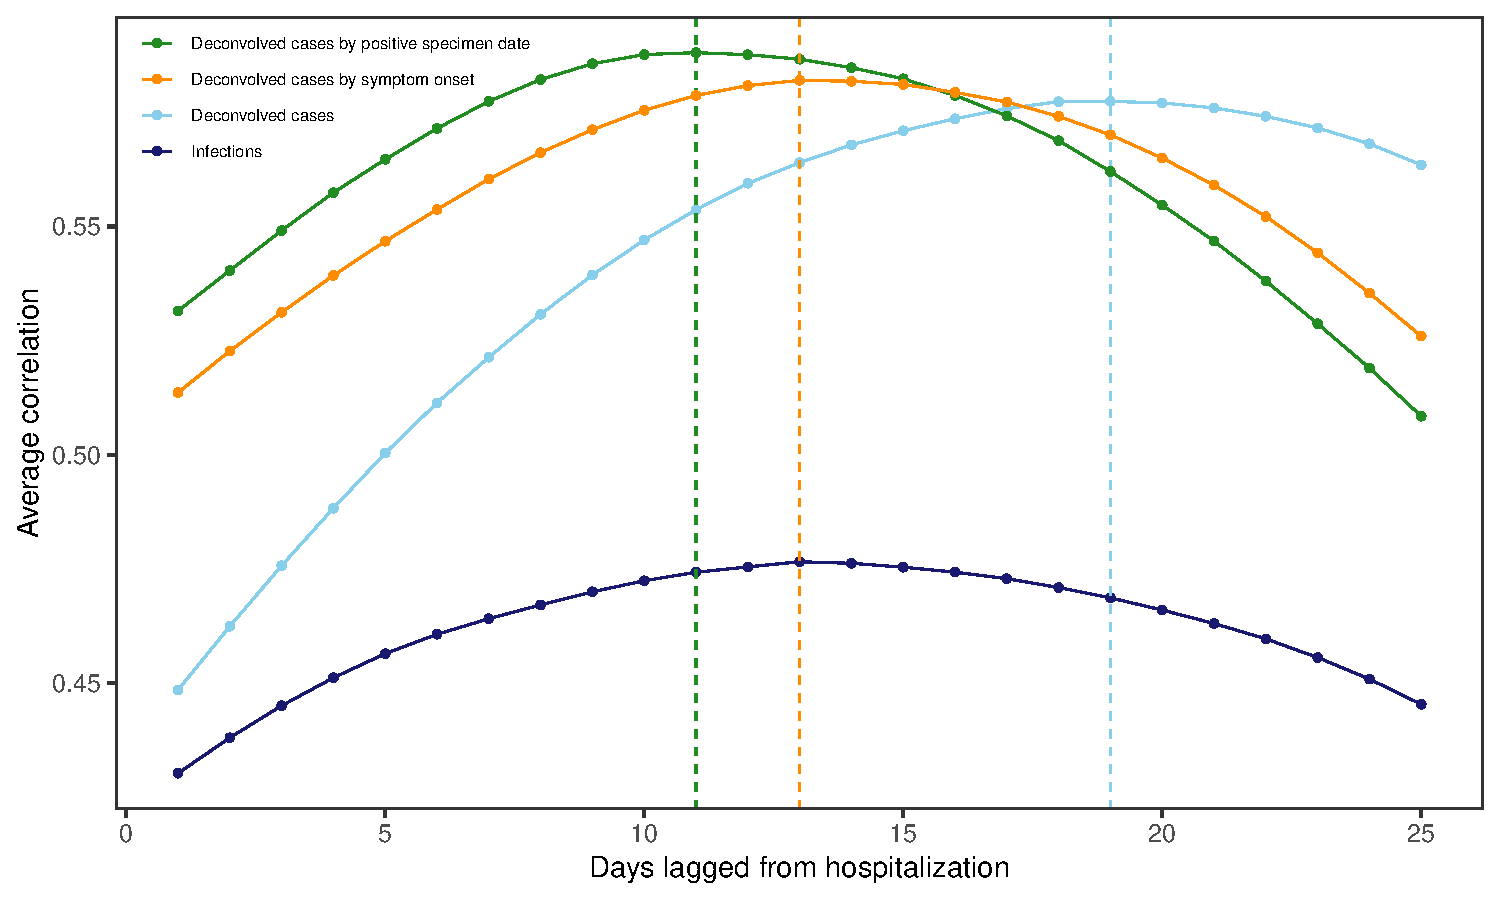
\includegraphics[width=.78\textwidth]{adj_unadj_pi_no_inc_hosp_lag_corr_F24.pdf} 
    \caption{Lagged Spearman's correlation between the infection and
    hospitalization rates per 100,000 averaged for each lag across \US states
    and days over June 1, 2020 to November 29, 2021, and taken over a rolling
    window of 61 days. The infection rates are based on the counts for the
    deconvolved case and infection estimates as well as the reported infections
    by symptom onset and when the report is symptom onset. Note that each such
    set of infection counts is subject to a center-aligned 7-day averaging to
    remove spurious day of the week effects. The dashed lines indicate the lags
    for which the highest average correlation is attained.}
    \label{fig:abl_lag_cor}
\end{figure}
 